\documentclass[conference]{IEEEtran}
\usepackage{graphicx}
\usepackage{amsfonts}
\usepackage{amssymb}
\usepackage[spanish]{babel}
\usepackage{verbatim}
\usepackage{amsbsy}
\usepackage{algorithm}
\usepackage{algorithmic}
\usepackage[T1]{fontenc}		%Previene errores en el encoding
\usepackage[utf8]{inputenc}		%para identificar acentos(encoding)
\usepackage{hyperref} %para url´s 
% correct bad hyphenation here
\usepackage{placeins} %para el FloatBarrier
\hyphenation{optical networks semiconductor IEEEtran}
\decimalpoint %decimales
\newtheorem{definition}{Definicion}[section]
\newtheorem{theorem}{Teorema}[section]
\newtheorem{lemma}{Lema}[section]

\begin{document}

% paper title
\title{Una aplicación del algoritmo Ncut, con una implementación open-source (en the R enviroment).  }


% author names and affiliations
% use a multiple column layout for up to three different
% affiliations
\author{\IEEEauthorblockN{J. Antonio García Ramírez}
\IEEEauthorblockA{Centro de Investigacion en Matematicas. Unidad Monterrey\\
jose.ramirez@cimat.mx}
}



% make the title area
\maketitle

\begin{abstract}
Si bien el analisis de datos es una tarea que ha cobrado el interés de la comunidad estadistica en años recientes y cuya familiaridad con el entorno de computo estadistico que el lenguaje R provee, alientan a la comunidad estadistica actual (nosotros alumnos y profesores del área) a realizar analisis estadistico completamente reproducible por medio de la herramienta R. \\
Si bien desde hace años existe una brecha entre el calculo de matrices en gran escala y el termino (referido como volumen) de “big data”, en este trabajo aplicamos el algoritmo de Normaliced Cut para segmentar imágenes. Pese a lo esperado el ambiente R posee pocas herramientas para analizar imágenes como lo podemos comprobar en la vista de la tarea ‘Medical Image Analysis’ \url{https://cran.r-project.org/web/views/MedicalImaging.html} en comparación a otras plataformas de computo como el ambiente del lenguaje Python o bien con software especializado como OpenCV \cite{OpenCV}.\\ 
Siendo notoria la ausencia de tal funcinamiento, en este trabajo compartimos una implementación del algoritmo Normalized Cut en el entorno de R con extensiones a programas y procesos realizados en C++, para proveer al usuario una amigable interfaz en R para segmentar imágenes. El articulo concluye evaluando la actual implementación y buscando formas de generalizar la implementación para un contexto de gran escala y reutilizar el codigo desarrollado.

\textit{Key words: Normaliced Cut, segmentación de imagenes, algoritmo de Lanczos, valores y vectores propios, grafo, matriz de similaridad, R (el ambiente de computo estadistico), open source, gran escala y big data.
}\end{abstract}

\IEEEpeerreviewmaketitle


\section{Introducción y motivación}
El reconocimiento estadistico de patrones, y en particular el analisis de imágenes, es un estimulante campo de estudio donde conviven la estadistica y las ciencias de la computación. En los años recientes el ambiente de computo estadistico y lenguaje de programación R \cite{R} ha aumentado su presencia en el análisis estadístico e inclusive es utilizado en contextos big data, por otro lado, el análisis de imágenes es un área que sigue motivando investigación.\\
En contrapunto de lo que se espera, pues el análisis de imágenes emplea diferentes técnicas de aprendizaje estadístico (tanto supervisado como no supervizado), el ambiente R posee pocas herramientas para análisis de imágenes como se puede comprobar al revisar la entrada de ‘MedicalImaging’ de su Task View,  frente a otras herramientas especializadas como OpenCV \cite{OpenCV}. Por su parte existen entornos de computo científico que integran algunas herramientas para analizar imágenes, pero sus capacidades se ven reflejadas en su precio comercial, por ejemplo MatLab \cite{MatLab}. \\
Lo anterior aunado al hecho de que la segmentación de imágenes es un objetivo final y a veces solo un paso intermedio en otras investigaciones, en el presente trabajo se desarrolla una aplicación de segmentación de imágenes utilizando el algoritmo Normalized Cut, al cual nos referiremos en lo siguiente como Ncut. Con el fin de proveer a los usuarios y desarrolladores del lenguaje R de una implantación del algoritmo Ncut (la cual no existe en OpenCV y otros entornos de computo científico) se codificaron dos programas; cada cual contiene un archivo con extensión .R que lo determina como codigo en lenguaje R al igual que un archivo con extensión .cpp que es codigo del lenguaje C++ que utiliza librerías estables del lenguaje C++ para efectuar cálculos y almacenamiento óptimo de matrices; uno para imágenes en escala de grises y otro para imágenes RGB disponibles en el github \cite{github} personal del autor \url{ https://github.com/fou-foo/MCE/tree/master/Second/AnalisisNumericoYOptimizacion/Miniproyecto } respectivamente los archivos son ‘W\_float.cpp’ y ‘mini\_cut\_float.R’ para imágenes en escala de grises y ‘W\_RGB\_float.cpp’ y ‘mini\_Ncut\_RGB\_float.R’ para imágenes en los canales RGB (el cual es fácilmente adaptable a imágenes con más canales). Detalles sobre la implementación se tratan en la última subsección de la sección 'III. Flujo de trabajo' de este reporte.\\
Con lo anterior se provee de una herramienta open-source fácil de usar en particular en el entorno R, aunque el codigo .cpp puede exportarse a otros entornos de cómputo, del algoritmo de Ncut lo cual sienta las bases de desarrollos de cómputo estadístico futuros. El producto desarrollado permitió segmentar un conjunto de imágenes del perfil personal del autor de la plataforma Facebook \cite{Facebook}, cuyos resultados son reportados en este trabajo.\\
La organización del presente trabajo es como sigue: en la sección ‘II. Flujo de trabajo’ se explica de manera general en que consiste el algoritmo Ncut que se utilizó en este trabajo, así como su relación con el algoritmo de Lanczos, posteriormente se detalla la implementación del algoritmo para que sea fácil de usar en el ambiente R.  En la sección ‘III. Trabajos relacionados y antecedentes’ reportamos la investigación realizada de la ausencia de implementaciones tanto del algoritmo Ncut como del algoritmo de Lanczos en diferentes arquitecturas (lo que hace tangible la necesidad de una implementación propia) como por ejemplo herramientas dedicadas al contexto big data (tales como Apache Hadoop \cite{Hadoop} y Apache Spark \cite{Spark}) en donde el autor ve un área de oportunidad para el analisis masivo de imágenes, por su parte en matrices de gran escala existen implementaciones en MPI como ScaLAPACK \cite{ScaLAPACK} del algoritmo de Lanczos sin embargo no implementan rutinas de mayor nivel como Ncut. Concluimos esa sección comentando sobre herramientas que a mediano plazo consideramos que serán de provecho para el computo científico a gran escala como el lenguaje de programación Elixir \cite{Elixir}. \\
Luego en la sección ‘IV. Experimentos y Resultados’ se muestran (y en algunas imágenes se detallan) los resultados de la segmentación de imágenes realizada con la implementación propia. La sección concluye con los beneficios y limitaciones de la implementación para obtener una “buena” segmentación de imágenes. Posteriormente en la sección ‘V. Conclusiones’ resumimos los descubrimientos aprendidos y evaluamos la metodología empleada. Finalmente, la sección ‘Apéndice’ plantea futuros trabajos de mejora de la implementación, dentro del contexto open-source, para segmentar imágenes de mayor resolución y tamaño a las abordadas en este trabajo, así como la posible extensión a otras técnicas de aprendizaje estadistico con la finalidad de reutilizar el codigo ya desarrollado y futuro.\\
\section{flujo de trabajo}

\subsection{Sobre el problema de segmentar de imágenes y enfoque de Ncut}
El problema de segmentar una imagen (considerando los valores que puede tener cada pixel en diferentes canales) se suele formular en términos matemáticos de la siguiente manera: dada una imagen cuyo conjunto de pixeles llamamos $V$, para sentar ideas un ejemplo consiste en tomar una imagen a colores en el espacio RGB donde cada pixel puede verse como la tripleta $(r,g,b)$ correspondiente a sus valores en cada canal, se busca particionar $V$ en conjuntos disjuntos $V_1,V_2,…V_m$ donde alguna medida de similaridad (es decir de parecido) entre los pixeles de cada $V_i$ es alta mientras la misma medida a través de conjunto diferentes $V_i$, $V_j$ es baja.\\
Si bien la anterior medida de similaridad responde a la importancia de percepciones visuales, espaciales y de agrupación ésta debe de ser compartida en pixeles próximos. En vista de que el conjunto de todas las posibles particiones de un conjunto $V$ es demasiado grande y crece exponencialmente como función de la cardinalidad de $V$, de hecho, esta es la definición de los números de Stirling del segundo tipo, surge la pregunta ¿Cómo escoger la partición “correcta” ?, de manera general existen dos maneras de abordar el problema: el primero consiste en prestar atención a niveles bajos de coherencia entre brillo, color y textura en cada pixel, sin embargo éste enfoque tiende a producir segmentaciones jerárquicas donde las jerarquías mayores responden a grupos y las menores a pixeles individuales, esto en la practica puede efectuarse con algoritmos computacionalmente costosos como los populares ‘single’ y ‘ward’ que producen dendogramas. En contraste el segundo enfoque de abordar el problema es el que comparte Ncut, el cual es un enfoque hacia abajo es decir que primero presta atención en áreas mayores y luego fijarse en los detalles, siguiendo la analogía de \cite{Ncut} “como un pintor primero marca las áreas grandes y después llena los detalles”.\\
Siguiendo las ideas de \cite{Ncut}, el problema de la segmentación de imágenes consiste en dos puntos: 
\begin{enumerate}
\item ¿Cuál es el criterio preciso para una buena partición?, es decir definir la similaridad entre elementos de $V$ 
\item ¿Cómo puede tal partición ser computada eficientemente?
\end{enumerate}  
De manera breve, el enfoque sugerido por \cite{Ncut}, para particionar una imagen consiste en considerar a los pixeles de una imagen $V$ como los vértices de una grafica $G=(V,E)$ y formar una partición en dos conjuntos $A$ y $B$ tales que $A \cup B = V$, $A \cap B = \emptyset $, simplemente removiendo aristas que conecten ambas partes. El grado de disimilaridad entre $A$ y $B$ puede calcularse como el peso total de las aristas que fueron removidas, en teoria de grafos esto es llamado \textit{corte}:
\[
cut(A,B) = \sum_{u\in A, v\in B} w(u,v)
\]
Encontrar el corte mínimo es un problema bien estudiado, inclusive en nivel licenciatura de carreras como matemáticas aplicadas o ciencias de la computación, y existen algoritmos eficientes para resolverlo. \\
Por otro lado \cite{Ncut} propone la siguiente medida de disociación entre grupos, el \textit{normalized cut} :
\[
Ncut(A,B)= \frac{cut(A,B)}{assoc(A,V)}+\frac{cut(A,B)}{assoc(B,V)}
\]
Donde $assoc(A, V) = \sum_{u\in A,t\in V}w(u,t)$ corresponde con el total de las conexiones de los nodos del conjunto $A$ a todos los nodos de la grafo y $assoc(B,V)$ es definido de manera similar. Un resultado fundamental de \cite{Ncut} es que minimizar la disociación a través de grupos, es decir la medida $Ncut$, es equivalente a maximizar la asociación dentro de cada grupo y que ambas condiciones pueden satisfacerse simultáneamente.   


\subsection{Aspectos matemáticos y computacionales}
Como es comentado en \cite{Ncut} encontrar el $Ncut$ optimo exactamente es un problema NP-completo (cuya elegante prueba se encuentra en el apéndice A del mismo paper \cite{Ncut} y es atribuida a Papadimitrou). Sin embargo, los autores de \cite{Ncut} prueban que relajar las condiciones al dominio continuo una solución aproximada al problema discreto puede encontrarse eficientemente y después de definir notación y con un poco de algebra los autores del paper muestran que esta solución aproximada a la minimización de $Ncut$ corresponde a:
\begin{equation}
\min_{\boldsymbol{x}}Ncut(\boldsymbol{x}) = \min_{\boldsymbol{y}} \frac{\boldsymbol{y}^t(D-W)\boldsymbol{y}}{\boldsymbol{y}^tD\boldsymbol{y}}
\end{equation}
Donde $ \boldsymbol{x}$ es un vector indicador con 1 en la i-ésima posición si el i-ésimo pixel se encuentra en $A$ y -1 en todas las otras $|V|-1$ entradas, $D=diag(d_1,d_2,…,d_{|V|})$ es la matriz diagonal donde $d_i=\sum_j w(i,j)$, $W$ es simplemente la matriz de pesos de las aristas es decir $W (i,j)=w_{ij}$, y finalmente $ \boldsymbol{y}$ es el vector donde cada entrada $i\in \{1,-b\}$ con $b = \frac{\sum_{x_i>0}d_i}{\sum_{x_i<0}d_i}$ y $ \boldsymbol{y}D \boldsymbol{1} = 0$ donde $ \boldsymbol{1}$ es un vector de dimensión $|V|$ con 1’s en todas sus entradas. \\
De lo anterior los autores de \cite{Ncut} reconocen que (1) corresponde con el cociente de Rayleigh \cite{MatrixC}. Relajando la condición de que $\boldsymbol{y}$
 tome valores reales (1) es minimizado por resolver el problema de valores propios generalizado:
\begin{equation}
(D-W)y = \lambda D y
\end{equation}
Como se demuestra en \cite{Ncut}  (2) es equivalente a el problema estándar de valores propios 
\begin{equation}
D^{-1/2}(D-W)D^{-1/2}z = \lambda z
\end{equation}
Donde $z=D^{1/2} y$. Una propiedad interesante de (3) es que $z_0= D^{1/2} \boldsymbol{1}$ es un vector propio asociado al valor propio 0 (lo cual es verificado en los experimentos efectuados), más aun $ D^{-1/2}(D-W)D^{-1/2}$ es simétrica y semi definida positiva, por lo que $z_0$ es el vector propio asociado al valor propio más pequeño y por el resultado espectral conocido de cursos de álgebra lineal, los vectores propios de una matriz son perpendiculares entonces el vector propio asociado al segundo valor propio más pequeño de (3) es perpendicular a $z_0$. Entonces el vector propio asociado al segundo valor propio más pequeño de (3) es la solución real de (2). \\
Tanto en la aplicación realizada en el conjunto de imágenes como en la implementación se utiliza explícitamente (3) para encontrar la partición deseada por medio de los valores y vectores propios correspondientes.\\
Como se expone en \cite{Ncut} existen varias peculiaridades sobre el uso del resultado anterior. Una imagen se puede segmentar utilizando los $k$ valores propios, y sus correspondientes vectores propios, más pequeños lo cual es computacionalmente costoso por las dimensiones de $W$ pues si la imagen original es de tamaño $h \times w$ entonces $W$ tiene dimensiones $(h\times w)\times (h\times w)$, o bien se puede partir de encontrar la primer solución de (3) y realizar el mismo procedimiento sobre cada conjunto $A$ y $B$ (lo cual es computacionalmente más eficiente, pues previamente ya se calculo la matriz $W$). En nuestra aplicación nuestro enfoque consistió en segmentar utilizando el vector propio asociado al segundo valor propio más pequeño de (3) para identificar dos grupos y tambien se consideró lo anterior en conjunto con el vector propio asociado al tercer valor propio más pequeño de (3) para segmentar en 3 conjuntos, en nuestro flujo de trabajo al obtener los dos vectores propios antes mencionados aplicamos el algoritmo de kmeans sobre las entradas de los vectores para tener grupos más definidos. Es importante mencionar que en vista de la naturaleza del algoritmo $Ncut$ la fase de preprocesamiento de las imágenes con las que se trabajó no contempla ningún filtro sobre la imagen original.   \\
Entonces el algoritmo de agrupación empleado en nuestra aplicación consiste en:\\
\begin{enumerate}
\item Dada una imagen de tamaño $h \times w$ con $n$ canales, considerada como un grafo $G=(V,E)$, construir la matriz de pesos $W$ conectando dos nodos con una medida de similaridad entre pares de nodos. Para lo cual elegimos un kernel gaussiano definido como 
\[
W_{ij}= e^{-||x_{(i)}-x_{(j)}||^2_2/2\sigma^2_I}e^{-||x_{(i)}-x_{(j)}||^2_2/2\sigma_x^2}
\] 
Si $||x_{(i)}-x_{(j)}||_2^2 < r^2$ y 0 en otro caso donde $x_{(i)}$ es el i-ésimo pixel de la imagen. En nuestros experimentos fijamos $\sigma_x^2=10$, $\sigma_I^2=0.05$ y siguiendo la recomendación de \cite{Ncut} fijamos $r = \left \lfloor
 \sqrt{\frac{(h\times w)-1}{2}*0.1}\right \rfloor +1 $, es decir que consideramos que cada pixel se conecta a lo más con $r^2$ pixeles alrededor de él en la métrica $L_2$.\\  
\item Resolver (3) y guardar los vectores propios asociados al segundo y tercer valor propios más pequeños 
\item Usar primero el vector propio asociado al segundo valor propio más pequeño y aplicar sobre sus entradas kmeans, posteriormente usar los dos vectores propios mencionados en el punto anterior y tambien utilizar kmeans sobre sus entradas para particionar la imagen en dos y tres conjuntos respectivamente.
\end{enumerate}
De manera general resolver el problema de valores propios para todos los valores propios requiere de $O(p^3)$ operaciones, donde $p$ es el numero de pixeles de la imagen (en nuestra notación $p = h \times w$), lo cual hace impráctico $Ncut$ para segmentación de imágenes grandes, sin embargo en nuestros experimentos logramos manejar imágenes hasta con 19200 pixeles (138 pixeles de cada lado para imágenes cuadradas), pero para nuestra aplicación en particular tenemos aspectos que favorecen el cómputo: primero nuestra matriz $W$ es simétrica (lo cual es consecuencia de la simetría del kernel usado) , semidefinida positiva y esparcida (en vista de la construcción de $r$) y solo requerimos de los vectores propios asociados a los tres valores propios más pequeños, como se menciona en \cite{Ncut} la precisión de los valores propios es baja pues como pudimos comprobar de manera experimental la distribución da las entradas de los vectores propios mencionados deja claro que con solo saber el signo correspondiente a la entrada del vector propio basta para clasificar y en adición a los comentarios de \cite{Ncut}  experimentalmente encontramos que el calculo de $W$ solo requiere de operaciones entre números de aritmética flotante del tipo \textit{float} en C++ en una arquitectura de 64bits. Las propiedades antes mencionadas son totalmente explotadas por el método de Lanczos, el cual tiene una complejidad de $O(mp)+O(mM(p))$ \cite{MatrixC} donde $m$ es el máximo número de cálculos del tipo matriz-vector (con matrices esparcidas) y $M(p)$ es el costo de la multiplicación de matriz-vector, como se trabaja con matrices esparcidas la complejidad de $M(p)$ es $O(p)$.\\   
Resumimos el flujo de trabajo que se siguió para segmentar imágenes usando Ncut en la figura 1. Donde el color azul indica que esa tarea se utilizo empleando en lenguaje R y el color naranja indica que la tarea se realizo por medio del lenguaje C++. En particular el preprocesamiento del segundo paso consistió en redimensionar las imágenes para que el número de pixeles en ellas no rebasara los 19,200 en los casos necesarios lo cual se realiza por medio de una interpolación de vecino más cercano con lo cual se pierde información de la imagen original pero hace factible la segmentación en este nuevo tamaño. Además de normalizar los valores de los pixeles en cada canal, es decir que en cada canal a cada valor de pixel se le resto el valor mínimo encontrado en el canal y se dividió el resultado entre el rango del canal original (diferencia entre el valor máximo y el mínimo).\\

\begin{figure}[htbp]
\center{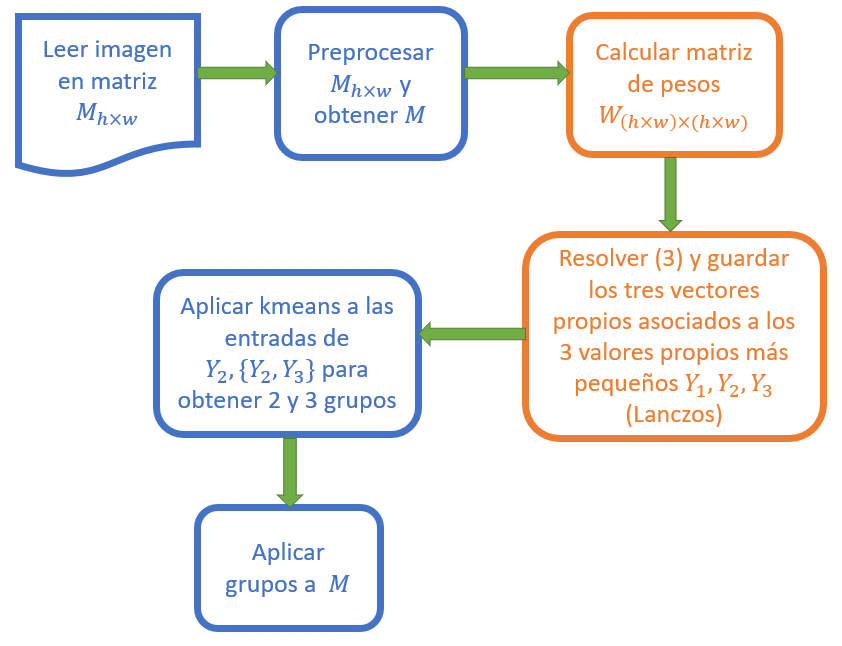
\includegraphics[width=7cm]{workflow.PNG}}
\caption{Flujo de trabajo para segmentar imagenes}
\label{workflow}
\end{figure}
\subsection{Detalles de la implementación (en particular en el lenguaje R)}
El lenguaje de programación R en particular posee retos en la aplicación del algoritmo \textit{Ncut} debido a las siguientes razones: 
\begin{enumerate}
\item La representación de las imágenes y en general de los números de punto flotante corresponden al estándar de \textit{double} del lenguaje C++
\item Carga en memoria RAM todos los objetos con los que se trabaja. 
\end{enumerate}
Sin embargo las matrices esparcidas son fáciles de manejar en el ambiente R.\\
Siguiendo el diagrama de la figura 1, la lectura de disco a RAM de cada imagen se realizó con el package \textit{imager} \cite{imager} el cual representa a las imágenes como un arreglo 4-dimensional donde las dos primeras dimensiones corresponden a la altura y ancho de la imagen respectivamente y la cuarta dimensión corresponde a los canales que dispone la imagen. Esta representación 4-dimensional emplea el tipo \textit{numeric} de R que corresponde al tipo de dato \textit{double} de C++ en 64 bits. En los casos en que se requirió redimensionar la imagen se realizo con el mismo package de R.\\
Para contrarrestar el punto (1) anterior el calculo de la matriz $W$ se realiza en C++ restringiendo el tipo de dato entre operaciones al tipo \textit{float}, para lo cual se emplea el package Rcpp \cite{Rcpp} y para almacenar la matrices en un formato de matriz esparcida se emplea el package RcppEigen \cite{RcppEigen} el cual permite interactuar con la libraría Eigen del lenguaje C++, de manera que la salida del codigo C++ es una matriz $W^*$ simétrica, semidefinida positiva y del tipo esparcida que incorpora la información necesaria para resolver el problema de valores propios de la ecuación (3). En particular el programa que segmenta imágenes con más de un canal emplea el package RcppArmadillo \cite{RcppArmadillo}, el cual a su vez es una interfaz para utilizar la librería de algebra lineal Armadillo de C++, para utilizar arreglos 3-dimensionales (en este punto es importante mencionar que la implementación actual requiere de efectuar cambios en el archivo header \textit{RcppArmadillo.h}, aumentando la línea ‘\#include <RcppEigen.h>’ pues la instalación default y el proceso de \textit{attach} innato del lenguaje R entran en conflicto el header \textit{RcppEigen.h} y \textit{RcppArmadillo.h} pues ambos hacen referencia al header \textit{Rcpp.h}, sin embargo al umentar la línea mencionada un solo header incluye a los demas en una sola invocaion y \textit{attachment}).\\ 
Hasta este punto utilizar el lenguaje C++ para el cálculo de $W$ mejoro notoriamente el tiempo de ejecución en comparación de hacerlo en R nato, además se ahorró espacio en memoria del 50\% al usar solo el tipo de dato \textit{float} en lugar de \textit{double} \\
Para contrarrestar el punto (2) de la lista anterior se remueven constantemente del ambiente de manera explícita los objetos que ya no se requieran y haciendo llamado explicito al \textit{garbage collector} de R así para el cuarto paso se emplea una función del package Rspectra \cite{RSpectra}, que es una interfaz a la librería Spectra desarrollada en C++ similar a la librería ARPACK (desarrollada en Fortran) , que hace referencia a una implementación en C++ del método de Lanczos reiniciado implícitamente y para obtener los valores propios más pequeños en lugar de los más grandes (que son la salida del método de Lanczos) se utiliza el método de shift alrededor del cero en lugar de invertir explícitamente la matriz $W^*$.\\
El quinto paso que consiste en aplicar kmeans sobre los vectores propios obtenidos previamente, se realizó con la implementación del kernel base de R con 50 iteraciones y fijando la semilla en ambos casos para proveer reproducibilidad al experimento, finalmente la aplicación de la segmentación corresponde a una convolución de matrices entre la imagen original, después de haber sido redimensionada en caso necesario, y el arreglo de los pixeles segmentados. En el caso de las imágenes con tres canales esta convolución mapea por canal a el valor original del pixel a cero, o bien lo multiplica por 0.5 o lo deja intacto dependiendo de a que segmento pertenece. 

\section{Trabajos relacionados}
En la sección anterior detallamos una implementación para segmentar imágenes usando el algoritmo \textit{Ncut} que depende fuertemente de la implementación del package RSpectra \cite{RSpectra} del método de Lanczos reiniciado implícitamente, el cual como ya mencionamos hace invocación a una versión implementada en C++ de su análogo en Fortran de la clásica librería ARPACK \cite{Arpack} para resolver el problema de encontrar los vectores propios asociados a los valores propios más pequeños de una matriz simétrica semidefinida positiva y esparcida. Sin embargo, la implementación actual esta limitada en cuanto a la dimensión de la matriz $W$ es por ello que recurrimos a redimensionar las imágenes de tamaño aproximadamente mayores a $138 \times 138$. \\
En un contexto de gran escala la librería ScaLAPACK \cite{ScaLAPACK} implementó una rutina que resuelve el problema de valores y vectores propios para el caso simétrico (como el que atacamos) sin embargo en un contexto big data existen implementaciones amigables, inclusive con una API al lenguaje Python (vease  \url{https://spark.apache.org/docs/2.3.0/mllib-dimensionality-reduction.html}), de la descomposición SVD (considerando a su vez solo los valores singulares más grandes) cuya implementación se detalla en \cite{MatrixSpark}, con este trabajo (y su actual implementación de la descomposición QR) o bien con la implementación de la inversa de una matriz en el ambiente Spark propuesta en \cite{Sparkbased} hacen plausible escalar el problema y la segmentación de imágenes usando el algoritmo \textit{Ncut} sin embargo, ello requiere de una nueva arquitectura. \\
Por otro lado esperamos que lenguajes de programación que nacen como funcionales y concurrentes como Elixir \cite{Elixir} lleguen a desarrollar librerías robustas para computo científico en el mediano plazo, pues al día de hoy el lenguaje cuenta con una librería de algebra lineal, sin embargo sigue en estado de desarrollo \cite{ElixirLib} como lo podemos comprobar al notar que su implementación de la inversa de una matriz ‘inv’ usa eliminación Gaussiana y fuerza bruta.   


\section{Experimentos y resultados}
La actual implementación que compartimos del algoritmo \textit{Ncut}, fue aplicada a un conjunto de imágenes del perfil de Facebook del autor. Los experimentos se reportan en el siguiente Cuadro I, haciendo referencia a cada imagen con un número  y el tiempo promedio de la ejecución en la imagen. Los experimentos se realizaron en una maquina Asus GL553VD con 8 GB de RAM (pero debido a la configuración del sistema operativo Windows 10) solo es posible utilizar completamente 6 de estos 8 GB, con un procesador Intel Core i7-7700HQ (con 8 núcleos físicos y lógicos) a una velocidad de 2.5GZ.\\
Durante los tiempos de ejecución, y parte del desarrollo, pudimos estimar la cantidad de memoria RAM que una PC requiere para ejecutar la actual implementación de \textit{Ncut}, la cual es aproximadamente 4 veces el espacio requerido para almacenar la matriz $W$, esto debido a que en algún punto se requiere de tener en memoria dos matrices adicionales a la matriz $W$ de las mismas dimensiones y mismas características, además de la memoria que utiliza la implementación de Lanzos para efectuarse.
\begin{table}[h]
\begin{center}
\begin{tabular}{c|cccccc}
\hline  \begin{tabular}{@{}c@{}}Número\\Nombre \\la imagen\end{tabular}  &\begin{tabular}{@{}c@{}}Tama\~no\\original\end{tabular}& \begin{tabular}{@{}c@{}}Tama\~no\\analizado\end{tabular} 
%(después de redimensionarla) 
& \begin{tabular}{@{}c@{}}Tiempo de\\ejecución\\ Gris\\(mins)\end{tabular} & \begin{tabular}{@{}c@{}}Tiempo de\\ejecución\\ RGB\\(mins)\end{tabular} &  \begin{tabular}{@{}c@{}}Tema\~no\\de matriz\\$W$\\(MB)\end{tabular}\\ \hline
1: Cell.jpg	     &100	$\times$ 69        & 100$\times$ 69 & 22.3 secs&	17.6 secs & 133.1\\
2: los\_amantes.jpg  &397 $\times$ 504     & 397$ \times$ 504   & 2.1 &2.4& 429.1\\
3: foo.jpg	&528 $\times$	528 &  132$\times$132	& 4.6&5.9 &855.2\\
4: guapa.jpg &970$\times$	720 & 100$\times$	180	&4.6& 4.9& 330.1\\
5: fer.jpg &533$\times$960 &100$\times$180 & 8.8 & 7.0 & 874\\
6: brindis.jpg	&1280$\times$960 & 160$\times$120 & 13.7 &7.1& 1000\\
7: foo\_clau.jpg &1280$\times$720&	104$\times$180 & 7.0& 8.1& 954.6\\
8: f002.jpg&960$\times$960&138 $\times$138& 16.9&8.9&1000\\
9: frascos.jpg&2048$\times$1152&180$\times$103&7.5&4.1&943.4\\
10: foo3.pjg&960$\times$960&138$\times$138&11.3&12.4&1000\\
%11: luis.jpg&2048$\times$1365&165$\times$110&3.8&10.2 &926.7\\
11: bicis.jpg&1280$\times$960& 160$\times$120&31.5&33.5&1000\\
%12: santa\_lucia.jpg&2048$\times$1152&182$\times$102&8.1&7.5&943.8\\
12: mariposa.jpg&2048$\times$1151&178$\times$100&5.9&3.3&863\\
13: filo\_liz.jpg&2048$\times$1152& 182$\times$102&7.9&7.0&943.8\\
14: marco.jpg&2048$\times$1365& 166$\times$110&5.4&4.7&933\\
\hline
\end{tabular}
\caption{Resumen de la ejecución del algoritmo \textit{Ncut} en el conjunto de imágenes muestra. Nótese que a partir de la imagen 2 todas las imágenes fueron redimensionadas.}
\label{tresultados}
\end{center}
\end{table}
\FloatBarrier
En la figura 2 (de arriba hacia abajo) se muestran los resultados obtenidos al segmentar las imágenes 1 a 5 utilizando ambos conjuntos de canales (escala de grises y RGB) después de ser redimensionadas a los tamaños descritos en el cuadro I. Es interesante remarcar que los resultados son buenos para las imágenes 1 y 5, por otro lado, para las imágenes 3 y 4 se logra identificar al mismo individuo, sin embargo en la imagen 2 al tratarse de la fotografía de un boceto a lápiz se identifican fácilmente las pinzas que sostienen al boceto y no es hasta la segmentación con dos vectores propios (derecha) que se identifica a todo el boceto como un solo conjunto diferenciándolo de las pinzas. \\
En la figura 3 (de arriba hacia abajo) se muestran los resultados obtenidos al segmentar las imágenes 6 a 10 utilizando de manera análogo a la figura 2. Es interesante remarcar que los resultados son consistentes al reconocer personas del fondo, por ejemplo la figura 10 y 8 (donde se detecta a la persona hasta en la segmentación que utiliza solo un vector propio y logrando mayor detalle al usar más componentes) sin embargo en la imagen 6 la segmentación en RGB solo es capaz de identificar la ropa de la persona de verde. Al visualizar la imagen 9 notamos que en particular la implementación es delicada reconociendo objetos de vidrio sin embargo distingue bien otros materiales como el plástico. En particular de los resultados de la figura 6 y 7 podemos apreciar que las condiciones de luz afectan el desempeño de la implementación lo que sugiere una mejora en el preprocesamiento para futuros trabajos.\\
\begin{figure}[htbp]
\center{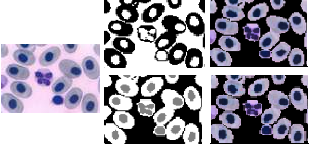
\includegraphics[width=6cm]{res_cel.png}}
\center{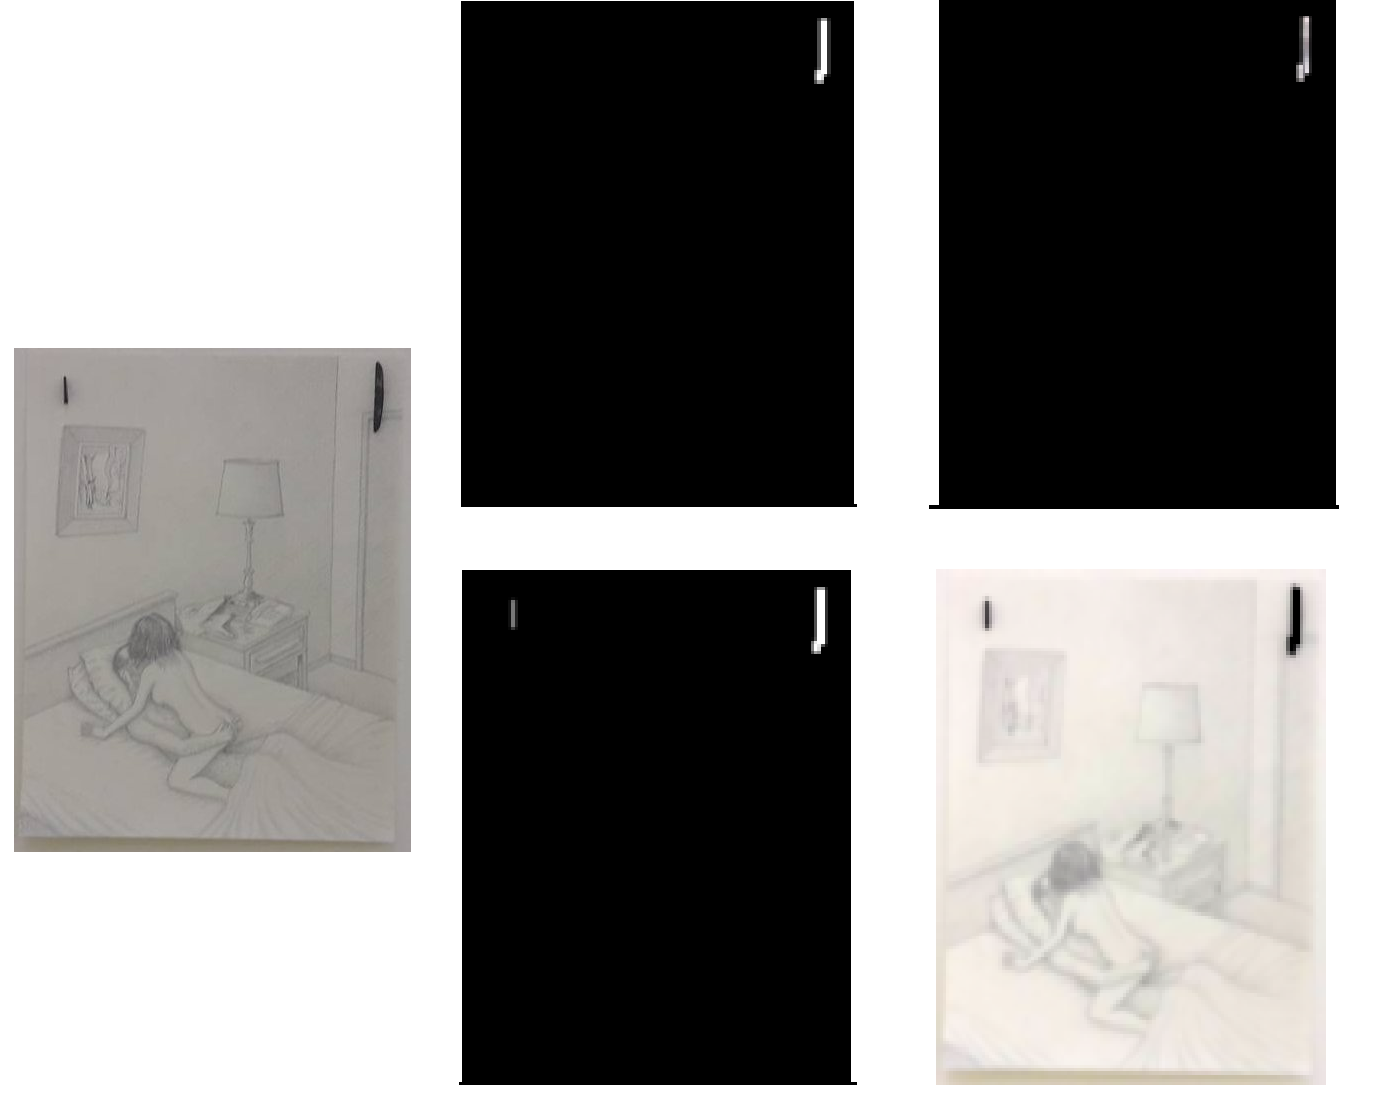
\includegraphics[width=6cm]{res_los_amantes.png}}
\center{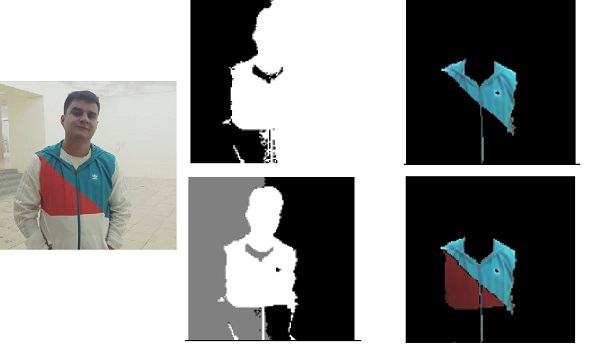
\includegraphics[width=6cm]{res_foo.jpg}}
\center{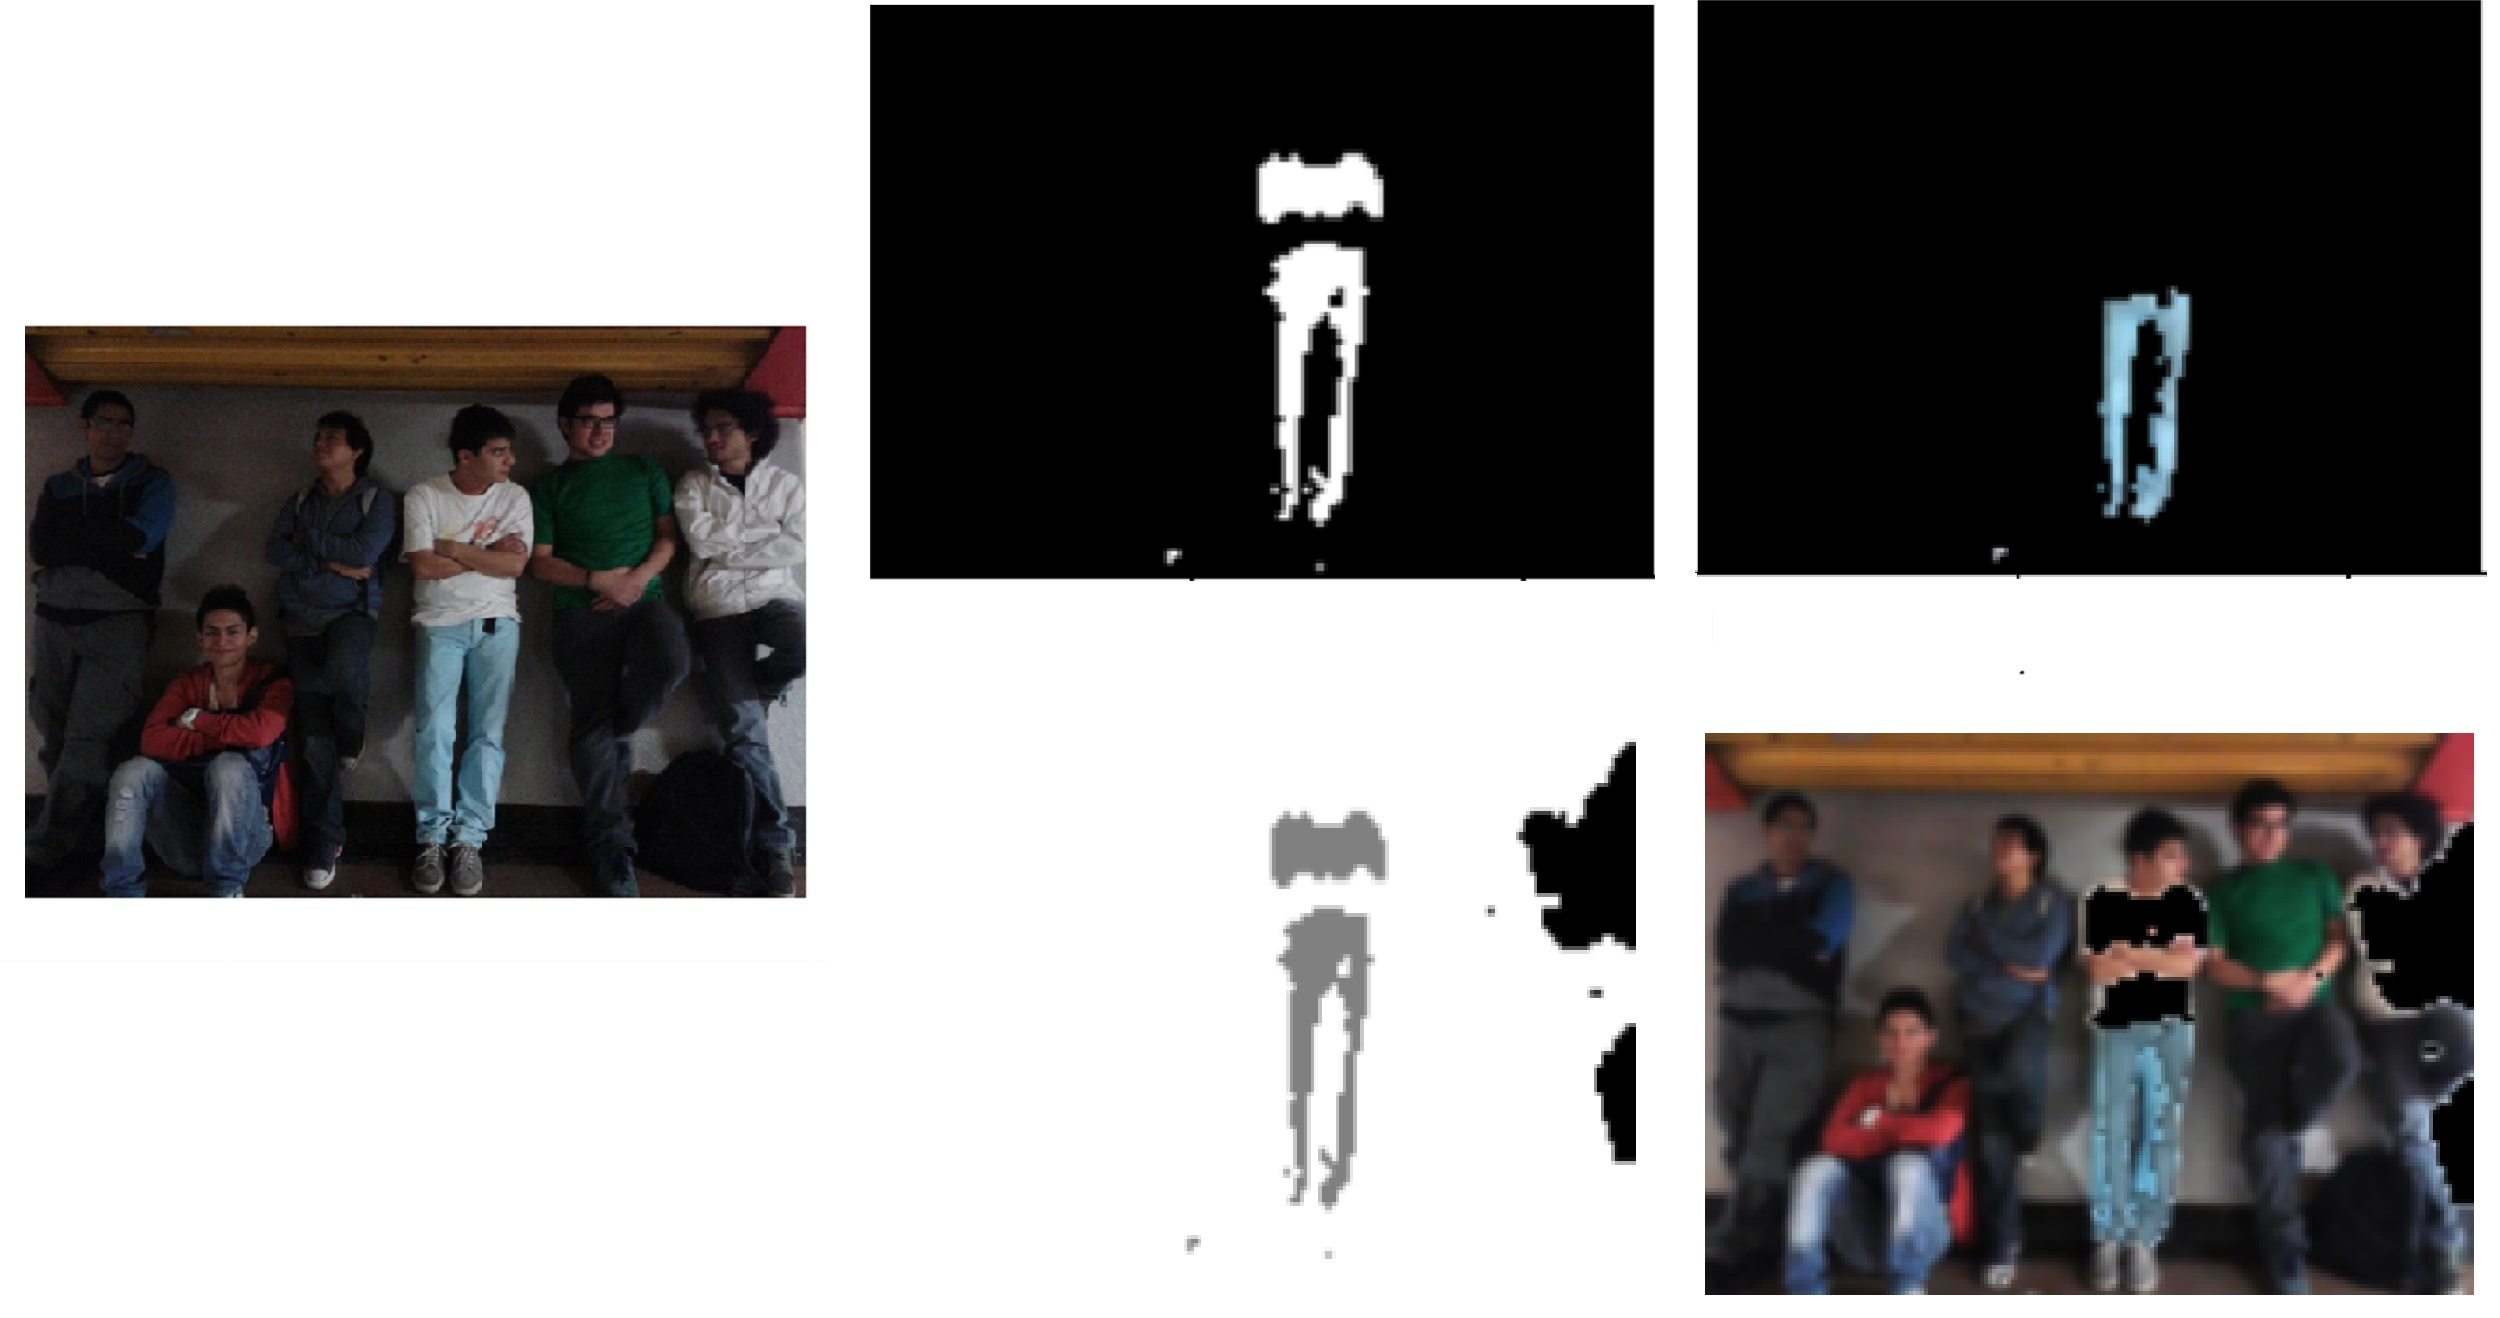
\includegraphics[width=6cm]{res_guapa.jpg}}
\center{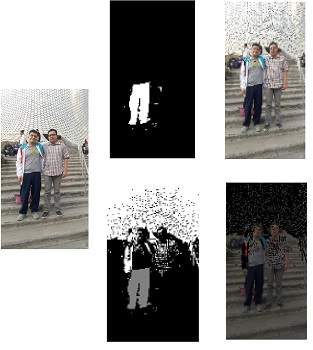
\includegraphics[width=6cm]{res_fer.jpg}}
\caption{Resultados de la segmentación de las imágenes 1 a 5, imagen original (izquierda), segmentación obtenida usando el vector propio asociado al segundo valor propio más pequeño en escala de grises y RGB (centro y derecha arriba) y segmentación obtenida usando los vectores propios asociados al segundo y tercer valor propio más pequeños en escala de grises y RGB (centro y derecha abajo)}
\label{res1}
\end{figure}
\FloatBarrier





\begin{figure}[htbp]
\center{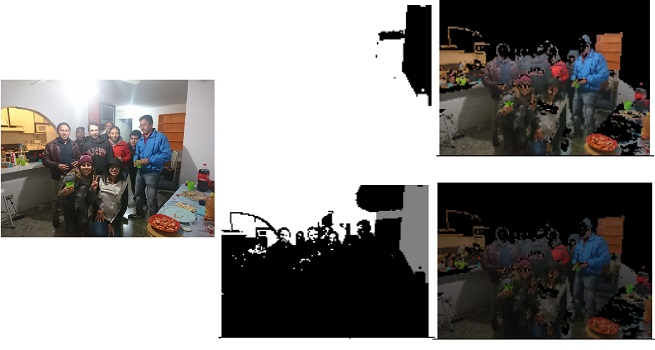
\includegraphics[width=6.3cm]{res_brindis.jpg}}
\center{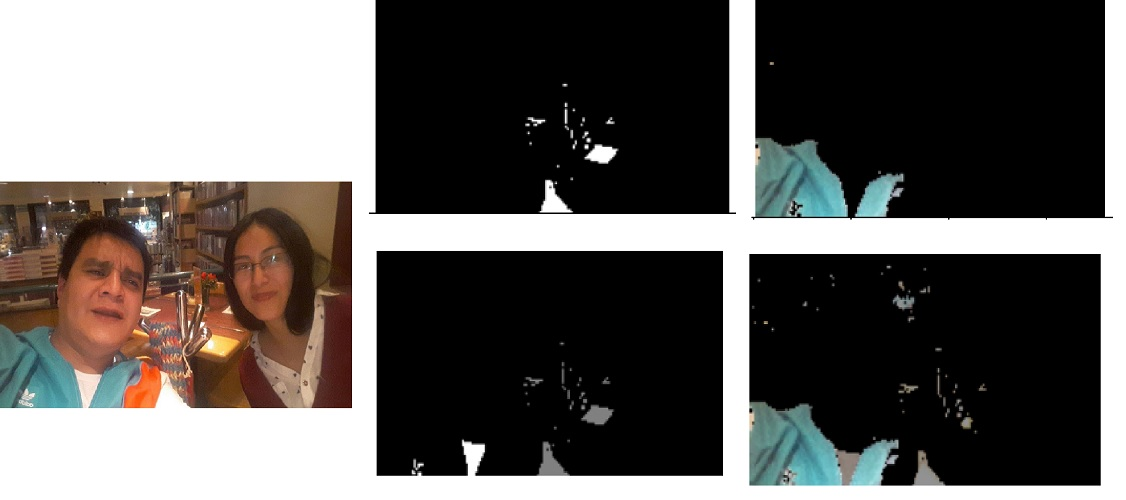
\includegraphics[width=6.3cm]{res_foo_clau.jpg}}
\center{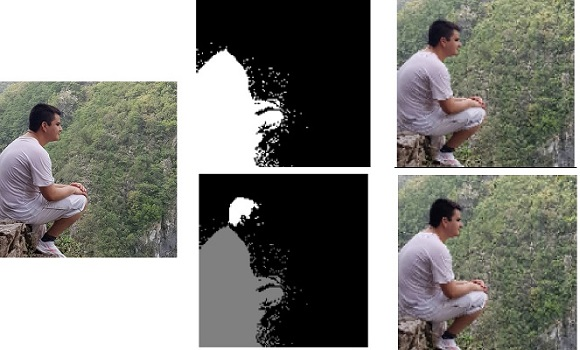
\includegraphics[width=6.3cm]{res_foo2.jpg}}
\center{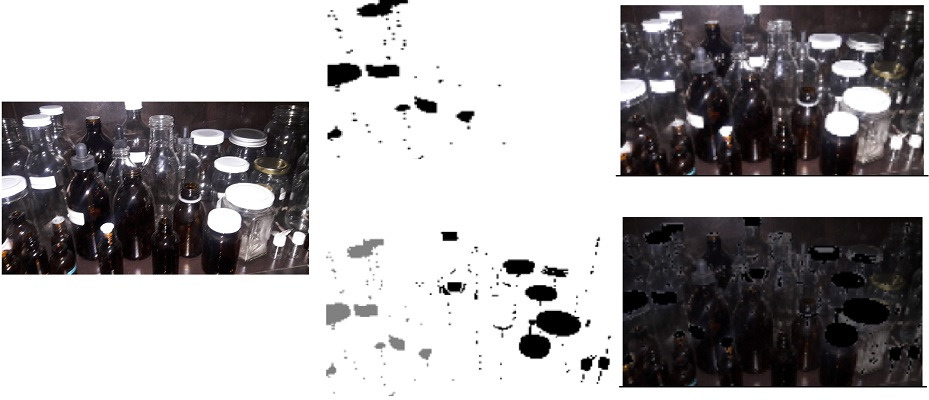
\includegraphics[width=6.3cm]{res_frascos.jpg}}
\center{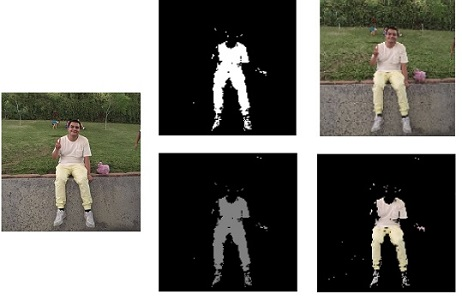
\includegraphics[width=6.3cm]{res_foo3.jpg}}
\caption{Resultados de la segmentación de las imágenes 11 a 14, imagen original (izquierda), segmentación obtenida usando el vector propio asociado al segundo valor propio más pequeño en escala de grises y RGB (centro y derecha arriba) y segmentación obtenida usando los vectores propios asociados al segundo y tercer valor propio más pequeños en escala de grises y RGB (centro y derecha abajo).}
\label{res2}
\end{figure}
\FloatBarrier
\newpage
En la figura 4 (de arriba hacia abajo) se muestran los resultados obtenidos al segmentar las imágenes 11 a 14 utilizando de manera análogo a la figura 2. Del anterior conjunto de imágenes concluimos: por un lado, la imagen 11 demuestra que (de manera ha doc a lo que esperábamos) la información que proporcionan los canales RGB es valiosa permitiendo identificar personas del fondo aun con un solo vector propio, en contrapunto las imágenes 12 y 13 logran un mayor desempeño en la escala de grises (aunque la imagen de la mariposa en los canales RGB se distingue fácilmente). Finalmente, la imagen 14 es otro boceto, pero a diferencia de la imagen 2, este es una fotografía, en donde vemos que la segmentación con dos canales en escala de grises logra un mejor desempeño al identificar el cuerpo sin embargo esto podría deberse a causas de iluminación a la hora de realizar la fotografía.


\begin{figure}[htbp]
\center{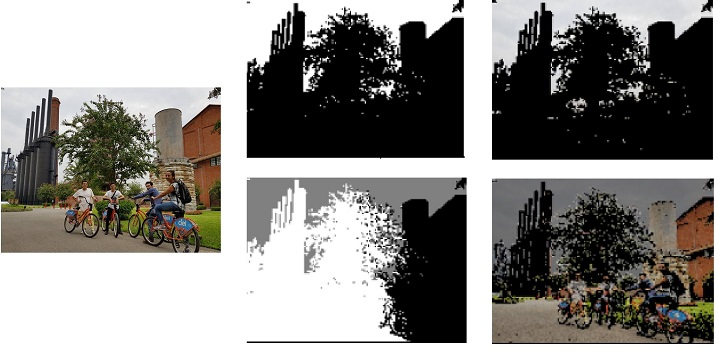
\includegraphics[width=6.65cm]{res_bicis.jpg}}
\center{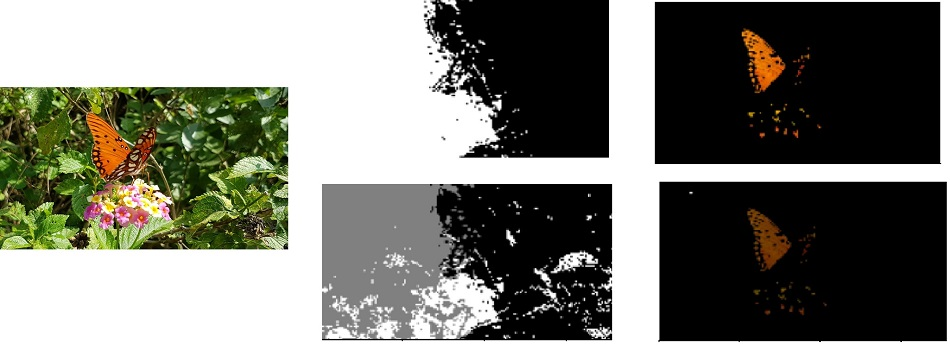
\includegraphics[width=6.6cm]{res_mariposa.jpg}}
\center{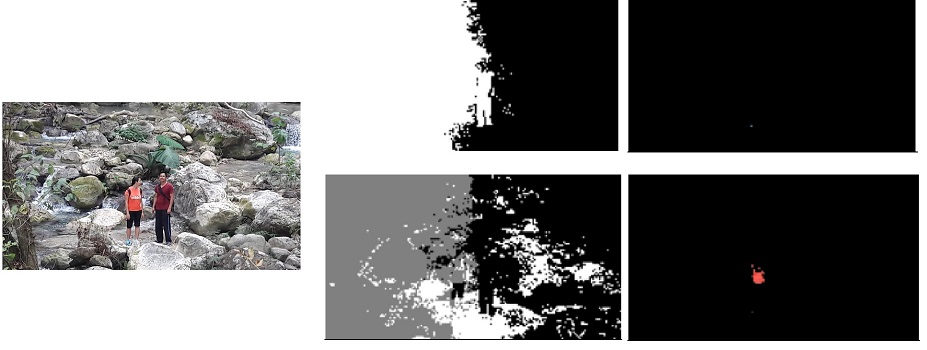
\includegraphics[width=6.6cm]{res_filo_liz.jpg}}
\center{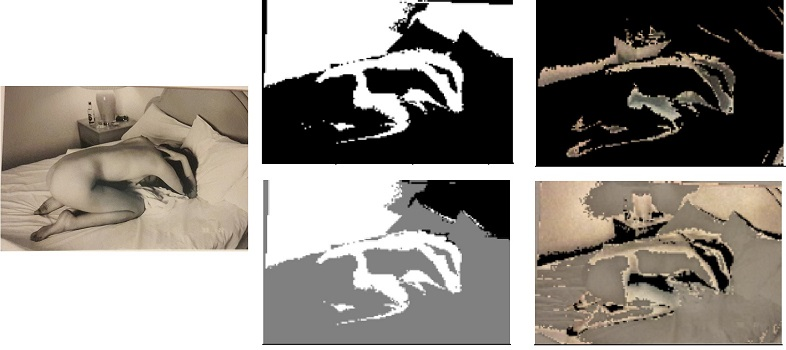
\includegraphics[width=6.65cm]{res_marco.jpg}}
\caption{Resultados de la segmentación de las imágenes 6 a 10, imagen original (izquierda), segmentación obtenida usando el vector propio asociado al segundo valor propio más pequeño en escala de grises y RGB (centro y derecha arriba) y segmentación obtenida usando los vectores propios asociados al segundo y tercer valor propio más pequeños en escala de grises y RGB (centro y derecha abajo).}
\label{res2}
\end{figure}
\FloatBarrier
\newpage

\section{Conclusiones}
De manera general lo aprendido en el desarrollo del presente trabajo es: el algoritmo \textit{Ncut} presenta gran potencial para segmentar imágenes (reconocer personas y variedad de materiales) como lo comprobamos en los experimentos. En analogía de otros muchos métodos de clasificación espectrales y basados en kernels, como \textit{string-kernels} o \textit{kernel PCA}, el algoritmo \textit{Ncut} \textbf{requiere de seleccionar "apropiadamente" un kernel} (en este caso la función que utilizamos para construir la \textbf{matriz de similaridad} $W$) \textbf{además de varios parámetros} (como las desviaciones estándar que involucra la definición del kernel usado, la manera de agrupar los pixeles a partir de vectores propios…). En contrapunto a los métodos mencionados \textit{Ncut} posee una \textbf{elegante} formulación que combina resultados básicos de algebra lineal y teoria de grafos y la NP-completes de su solución exacta, lo hacen atractivo y \textit{nos anima a trabajos posteriores} para \textbf{evadir} el paso en el preprocesamiento que consistió en \textbf{redimensionar la imagen}.



\section*{Apéndice}

\subsection*{Trabajos futuros}
Como trabajos futuros, en primera instancia consideramos evadir la redimensionar de las imágenes y con ello experimentar si considerar la imagen en su totalidad aporta información que valga el desarrollo e implementación en gran escala (en el corto plazo consideramos expandir la implementación para que considere inputs de 3000$\times$3000) a pesar de que ello implique mover la arquitectura de computo usada. \\
Con lo anterior mejoraremos los tiempos de ejecución y consideramos la opción de afinar los parámetros que mencionamos en la sección anterior en el algoritmo con el fin de obtener mejores resultados y en el mediano plano realizar hipótesis acerca de la distribución de tales parámetros en diferentes dominios, o conjuntos, de imágenes. 


%\begin{displaymath}
%[y]^- = -yI(-y) \textrm{, con } I(-y)=\left\lbrace 
%	\begin{array}{cc}
%	1	&	\textrm{ si } y < 0	\\
%	0	&	\textrm{ otro caso}
%	\end{array} \right.
%\end{displaymath}


%\begin{algorithm}
%{\footnotesize
%\caption{Quadratic Penalty}
%\label{algQuadPen}
%\begin{algorithmic}[1]
%\STATE Given $(\mu_0 > 0$, tolerance $\tau_0$, starting point $x_0^s$
%\FOR{$k=0,1,2\ldots$}
%\STATE Find an approximate minimizer $x_k$ of $Q(\cdot;\mu_k)$, starting at $x_k^s$, and terminating when $||\nabla Q(x;\mu_k)||\leq \tau_k$
%\IF{final convergence test satisfied}
%\STATE \textbf{STOP} with approximate solution $x_k$
%\ENDIF
%\STATE Choose new penalty parameter $\mu_{k+1} \in (0,\mu_k)$
%\STATE Choose new starting point $x_{k+1}^s$
%\ENDFOR
%\end{algorithmic}}
%\end{algorithm}



%{\footnotesize
%\begin{eqnarray}\label{eqgrad}
%\nabla_x \mathcal{L}_A(x_k,\lambda^k;\mu_k) & = & \nabla f(x_k) - \sum_{i\in \mathcal{I}|c_i(x)\leq\mu\lambda_i^k} \left(\lambda_i^k - \frac{c_i(x_k)}{\mu_k} \right) \nabla c_i(x_k)	\nonumber \\
%\end{eqnarray}
%}


%\begin{table}[htbp]
%\begin{center}
%\begin{tabular}{|c|c|c|c|}
%\hline
%			& Penalizaci\'on Cuadr\'atica		&	Barrera Logar\'itmica	&	Lagrangiano Aumentado	\\
%\hline
%$f(x^{*})$	& 0.1643	&	0.1774	&	0.1642	\\
%\hline
%\end{tabular}
%\caption{Resultados para cada m\'etodo en el problema a optimizar.}
%\label{tresults1}
%\end{center}
%\end{table}
\newpage
\begin{thebibliography}{1}
\bibitem{Arpack}
Richard B Lehoucq, Danny C Sorensen, and Chao Yang, \textit{ARPACK users' guide: solution of large-scale eigenvalue problems with implicitly restarted Arnoldi methods}, volume 6. Siam, 1998.

\bibitem{Elixir}
Desarrollado por José Valim para Plataformatec, \emph{Elixir} , \url{https://elixir-lang.org/}
\bibitem{Facebook}
Facebook Inc, \emph{Facebook}, 2018 y \url{https://www.facebook.com/}

\bibitem{github}
GitHub ,Inc., \emph{GitHub}, 2018 y \url{https://github.com/}

\bibitem{MatrixC}
G.H. Golub and C.F. Van Loan, \emph{Matrix Computations}, John
Hopkins Press, 1989.

\bibitem{MatrixSpark}
Bosagh Zadeh, Reza and Meng, Xiangrui and Ulanov, Alexander and Yavuz, Burak and Pu, Li and Venkataraman, Shivaram and Sparks, Evan and Staple, Aaron and Zaharia, Matei; \textit{Matrix Computations and Optimization in Apache Spark}, Proceedings of the 22Nd ACM SIGKDD International Conference on Knowledge Discovery and Data Mining, KDD '16 2016, ISBN:978-1-4503-4232-2; San Francisco, California, USA; pags 31--38,
\url{http://doi.acm.org/10.1145/2939672.2939675}


\bibitem{Hadoop}
'Welcome to Apache Hadoop!',  \emph{Welcome to Apache Hadoop!}, \url{http://hadoop.apache.org/}. Consultado: 31-Mar-
2018.

\bibitem{imager}
Simon Barthelme (2017). \emph{imager: Image Processing
  Library Based on 'CImg'}, R package versión  0.40.2., \url{  https://CRAN.R-project.org/package=imager}

\bibitem{MatLab} 
The MathWorks Inc., \emph{MATLAB}; Natick, Massachusetts, año 2000

\bibitem{ElixirLib}
 Friedel Ziegelmayer, \emph{Matrix}; \url{https://hexdocs.pm/matrix/Matrix.html#summary}, consultado el 15 de abril de 2018.


\bibitem{OpenCV}
Bradski, G., \emph{The OpenCV Library}, journal Dr. Dobb's Journal of Software Tools id:2236121, 2008-01-15, año 2000 

\bibitem{R}
R Core Team, \emph{R: A Language and Environment for Statistical Computing}, R Foundation for Statistical Computing; Vienna, Austria, 2014 y  \url = {http://www.R-project.org/}

\bibitem{Rcpp}
Dirk Eddelbuettel and James Joseph Balamuta (2017). \emph{Extending R with C++: A Brief Introduction to Rcpp}. PeerJ Preprints 5:e3188v1, \url{https://doi.org/10.7287/peerj.preprints.3188v1.}

\bibitem{RcppArmadillo}
Dirk Eddelbuettel, Conrad Sanderson (2014), \emph{RcppArmadillo: Accelerating R with
  high-performance C++ linear algebra}, Computational Statistics and Data Analysis,
  Volume 71, March 2014, pages 1054-1063. URL
  http://dx.doi.org/10.1016/j.csda.2013.02.005

\bibitem{RcppEigen}
Douglas Bates, Dirk Eddelbuettel (2013), \emph{Fast and Elegant Numerical Linear Algebra Using the RcppEigen Package}, Journal of Statistical Software, 52(5), 1-24. \url{http://www.jstatsoft.org/v52/i05/}

\bibitem{RSpectra}
Yixuan Qiu and Jiali Mei (2016), \emph{RSpectra: Solvers for Large Scale Eigenvalue and SVD Problems}, R package version 0.12-0, \url{https://CRAN.R-project.org/package=RSpectra}

\bibitem{ScaLAPACK}
Blackford, L. S. and Choi, J. and Cleary, A., D'Azevedo, E. and Demmel, J. and Dhillon, I. and Dongarra, J. and Hammarling, S. and Henry, G. and Petitet, A. and Stanley, K. and Walker, D. and Whaley, R. C.;\emph{ScaLAPACK Users' Guide}, Society for Industrial and Applied Mathematics 1997,
Philadelphia, PA. ISBN :0-89871-397-8  

\bibitem{Ncut}
Shi J. and Malik J., \emph{Normalized Cuts and Image Segmentation}, IEEE Transactions on pattern analysis and machine learning, VOL. 22, No. 8, Agosto 2000.

\bibitem{Spark}
Spark Community. \emph{Apache Spark},  \url{https://spark.apache.org/}. Consultado: 31-Mar-2018

\bibitem{Sparkbased}
J. Liu, Y. Liang and N. Ansari; \emph{Spark-Based Large-Scale Matrix Inversion for Big Data Processing}; IEEE Access, vol. 4, pp. 2166-2176, 2016, \url{http://ieeexplore.ieee.org/stamp/stamp.jsp?tp=&arnumber=7440788&isnumber=7419931}

\end{thebibliography}


\end{document}

